\documentclass[14pt]{beamer}
\usepackage{./Estilos/BeamerUVM}
\usepackage{./Estilos/ColoresLatex}
%Sección para el tema de beamer, con el theme, usercolortheme y sección de footers
\usetheme{Berlin}
\usecolortheme{beaver}
%\useoutertheme{default}
\setbeamercovered{invisible}
% or whatever (possibly just delete it)
\setbeamertemplate{section in toc}[sections numbered]
\setbeamertemplate{subsection in toc}[subsections numbered]
\setbeamertemplate{subsection in toc}{\leavevmode\leftskip=3.2em\rlap{\hskip-2em\inserttocsectionnumber.\inserttocsubsectionnumber}\inserttocsubsection\par}
% \setbeamercolor{section in toc}{fg=blue}
% \setbeamercolor{subsection in toc}{fg=blue}
% \setbeamercolor{frametitle}{fg=blue}
% \setbeamertemplate{caption}[numbered]

\setbeamertemplate{footline}
\beamertemplatenavigationsymbolsempty
\setbeamertemplate{headline}{}


\makeatletter
% \setbeamercolor{section in foot}{bg=gray!30, fg=black!90!orange}
% \setbeamercolor{subsection in foot}{bg=blue!30!yellow, fg=red}
% \setbeamercolor{date in foot}{bg=black, fg=white}
\setbeamertemplate{footline}
{
  \leavevmode%
  \hbox{%
  \begin{beamercolorbox}[wd=.333333\paperwidth,ht=2.25ex,dp=1ex,center]{section in foot}%
    \usebeamerfont{section in foot} \insertsection
  \end{beamercolorbox}%
  \begin{beamercolorbox}[wd=.333333\paperwidth,ht=2.25ex,dp=1ex,center]{subsection in foot}%
    \usebeamerfont{subsection in foot}  \insertsubsection
  \end{beamercolorbox}%
  \begin{beamercolorbox}[wd=.333333\paperwidth,ht=2.25ex,dp=1ex,right]{date in head/foot}%
    \usebeamerfont{date in head/foot} \insertshortdate{} \hspace*{2em}
    \insertframenumber{} / \inserttotalframenumber \hspace*{2ex} 
  \end{beamercolorbox}}%
  \vskip0pt%
}

% \usefonttheme{serif}
\usepackage[clock]{ifsym}
\DeclareSIUnit\erg{erg}
\DeclareSIUnit[number-unit-product = {\,}]\cal{cal}

\sisetup{per-mode=symbol}
\resetcounteronoverlays{saveenumi}

% Macro para agregar el logo de UVM en cada slide de la presentación

\addtobeamertemplate{frametitle}{}{%
\begin{tikzpicture}[remember picture,overlay]
\coordinate (logo) at ([xshift=-1.5cm,yshift=-0.8cm]current page.north east);
% \fill[devryblue] (logo) circle (.9cm);
% \clip (logo) circle (.75cm);
\node at (logo) {
\includegraphics[width=2.1cm]{Imagenes/logo_UVM.png}};
\end{tikzpicture}}


\title{\Large{Transformaciones de Energía} \\ \normalsize{Física III}}
\date{}

\begin{document}
\maketitle

\section*{Contenido}
\frame[allowframebreaks]{\frametitle{Contenido} \tableofcontents[currentsection, hideallsubsections]}

\section{Transformaciones de energía}
\frame{\tableofcontents[currentsection, hideothersubsections]}
\subsection{Energía constante}

\begin{frame}
\frametitle{¿Qué son las transformaciones?}
Las \textocolor{carnelian}{transformaciones de energía} se refieren a los cambios en la forma de la energía en un sistema.
\end{frame}
\begin{frame}
\frametitle{Conservación de energía}
La energía no se crea ni se destruye, pero puede cambiar de una forma a otra.
\end{frame}

\subsection{Tipos de transformaciones}

\begin{frame}
\frametitle{Transf. de Energía Mecánica}
Cuando levantas un objeto, realizas trabajo mecánico. 
\begin{figure}
    \centering
    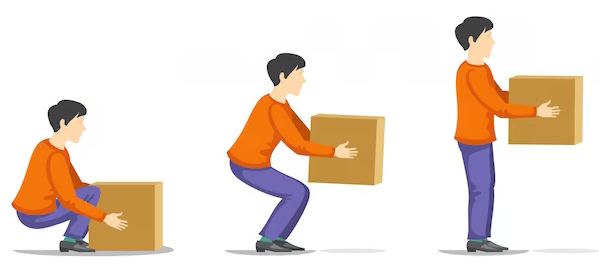
\includegraphics[scale=0.25]{Imagenes/Transformacion_Energia_01.png}
\end{figure}
\end{frame}
\begin{frame}
\frametitle{Transf. de Energía Mecánica}
La energía potencial mecánica en el objeto se convierte en energía cinética a medida que cae.
\end{frame}
\begin{frame}
\frametitle{Transf. de Energía Térmica (Calor)}
\vspace*{-1cm}
Al frotar tus manos.
\pause
\begin{figure}
    \centering
    
\includegraphics[scale=2.5]{Imagenes/Transformacion_Energia_02.jpg}
\end{figure}
La energía mecánica se transforma en calor debido a la fricción.
\end{frame}
\begin{frame}
\frametitle{Transf. de Energía Eléctrica}
\vspace*{-1cm}
En una lámpara.
\pause
\begin{figure}
    \centering
    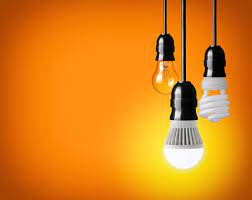
\includegraphics[scale=0.5]{Imagenes/Transformacion_Energia_03.jpg}
\end{figure}
La energía eléctrica se transforma en energía luminosa y térmica.
\end{frame}
\begin{frame}
\frametitle{Transf. de Energía Luminosa}
\vspace*{-1cm}
Cuando enciendes una linterna.
\pause
\begin{figure}
    \centering
    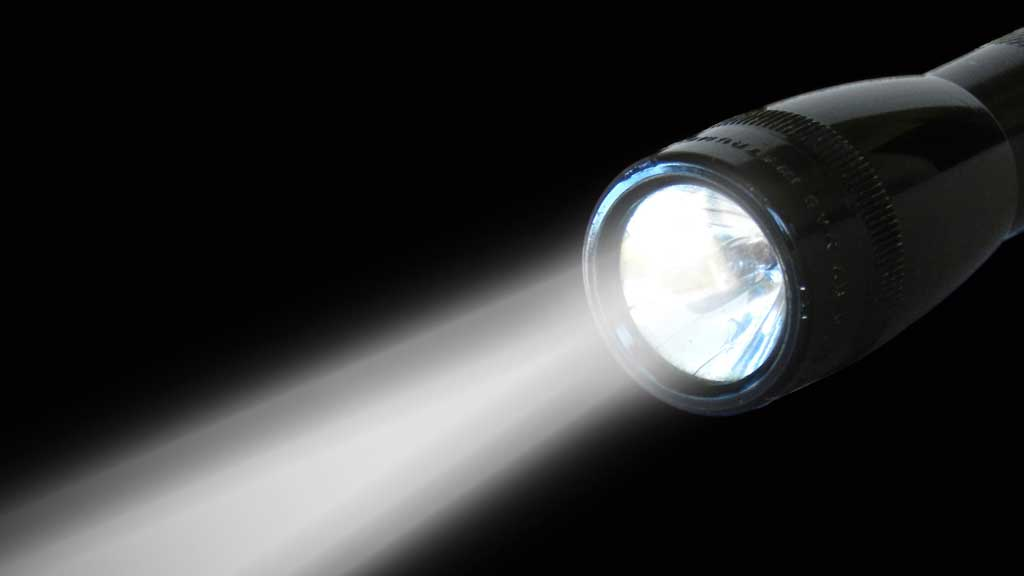
\includegraphics[scale=0.2]{Imagenes/Transformacion_Energia_04.jpg}
\end{figure}
La energía eléctrica se transforma en energía luminosa.
\end{frame}
\begin{frame}
\frametitle{Transf. de Energía Química}
\vspace*{-1cm}
Durante la digestión de alimentos.
\pause
\begin{figure}
    \centering
    
\includegraphics[scale=0.25]{Imagenes/Transformacion_Energia_05.jpg}
\end{figure}
\end{frame}
\begin{frame}
\frametitle{Transf. de Energía Química}
La energía química almacenada en los nutrientes se transforma en energía térmica y mecánica.
% 6. Transformación de Energía Sonora:
% Ejemplo: Al golpear un tambor, la energía mecánica se transforma en energía sonora.
% 7. Transformación de Energía Nuclear:
% Ejemplo: En una central nuclear, la energía nuclear se transforma en energía térmica, que luego se utiliza para generar electricidad.
% 8. Transformación de Energía Cinética:
% Ejemplo: Cuando un vehículo frena, la energía cinética se transforma en energía térmica debido a la fricción de los frenos.
% 9. Transformación de Energía Potencial:
% Ejemplo: Al soltar un resorte comprimido, la energía potencial elástica se convierte en energía cinética.
% 10. Transformación de Energía Solar:
% Ejemplo: Los paneles solares transforman la energía solar en energía eléctrica.
% 11. Transformación de Energía Hidráulica:
% Ejemplo: Una presa hidroeléctrica transforma la energía potencial del agua en energía eléctrica.
% 12. Transformación de Energía Eólica:
% Ejemplo: Un aerogenerador convierte la energía cinética del viento en energía eléctrica.
% 13. Transformación de Energía de Marea:
% Ejemplo: Las instalaciones de energía de marea transforman la energía de las mareas en electricidad.
% 14. Transformación de Energía Magnética:
% Ejemplo: Un generador eléctrico puede transformar la energía magnética en energía eléctrica.
% 15. Transformación de Energía Potencial Gravitatoria:
% Ejemplo: Una montaña rusa transforma la energía potencial gravitatoria en energía cinética y viceversa.
% Estos ejemplos ilustran cómo la energía puede cambiar de una forma a otra, y a menudo, en la práctica, hay múltiples transformaciones de energía que ocurren en un sistema. Estas transformaciones son fundamentales para comprender el funcionamiento de diversos dispositivos y sistemas en la vida cotidiana y en la industria.
\end{frame}




\end{document}